\chapter{نتیجه و بحث}
در اولین جلسه از آزمایشگاه مدارهای منطقی با کار با سه نرم‌افزار مهم آشنا شدیم.

\begin{figure}[h]
\centering

\includegraphics[scale=0.4]{conclusion/fritzing.png}
\caption{
لوگوی نرم‌افزار
Fritzing}
\end{figure}

نرم‌افزار اول
Fritzing
بود که اوپن‌سورس است ولی قابلیت‌های چندانی از جمله شبیه‌سازی ندارد و تنها برای طراحی مدارات و قطعات است. البته از مزیت‌های این برنامه نزدیک به واقعیت بودن قطعات است و این امر برای طراحی بسیار مناسب است.

\begin{figure}[h]
\centering
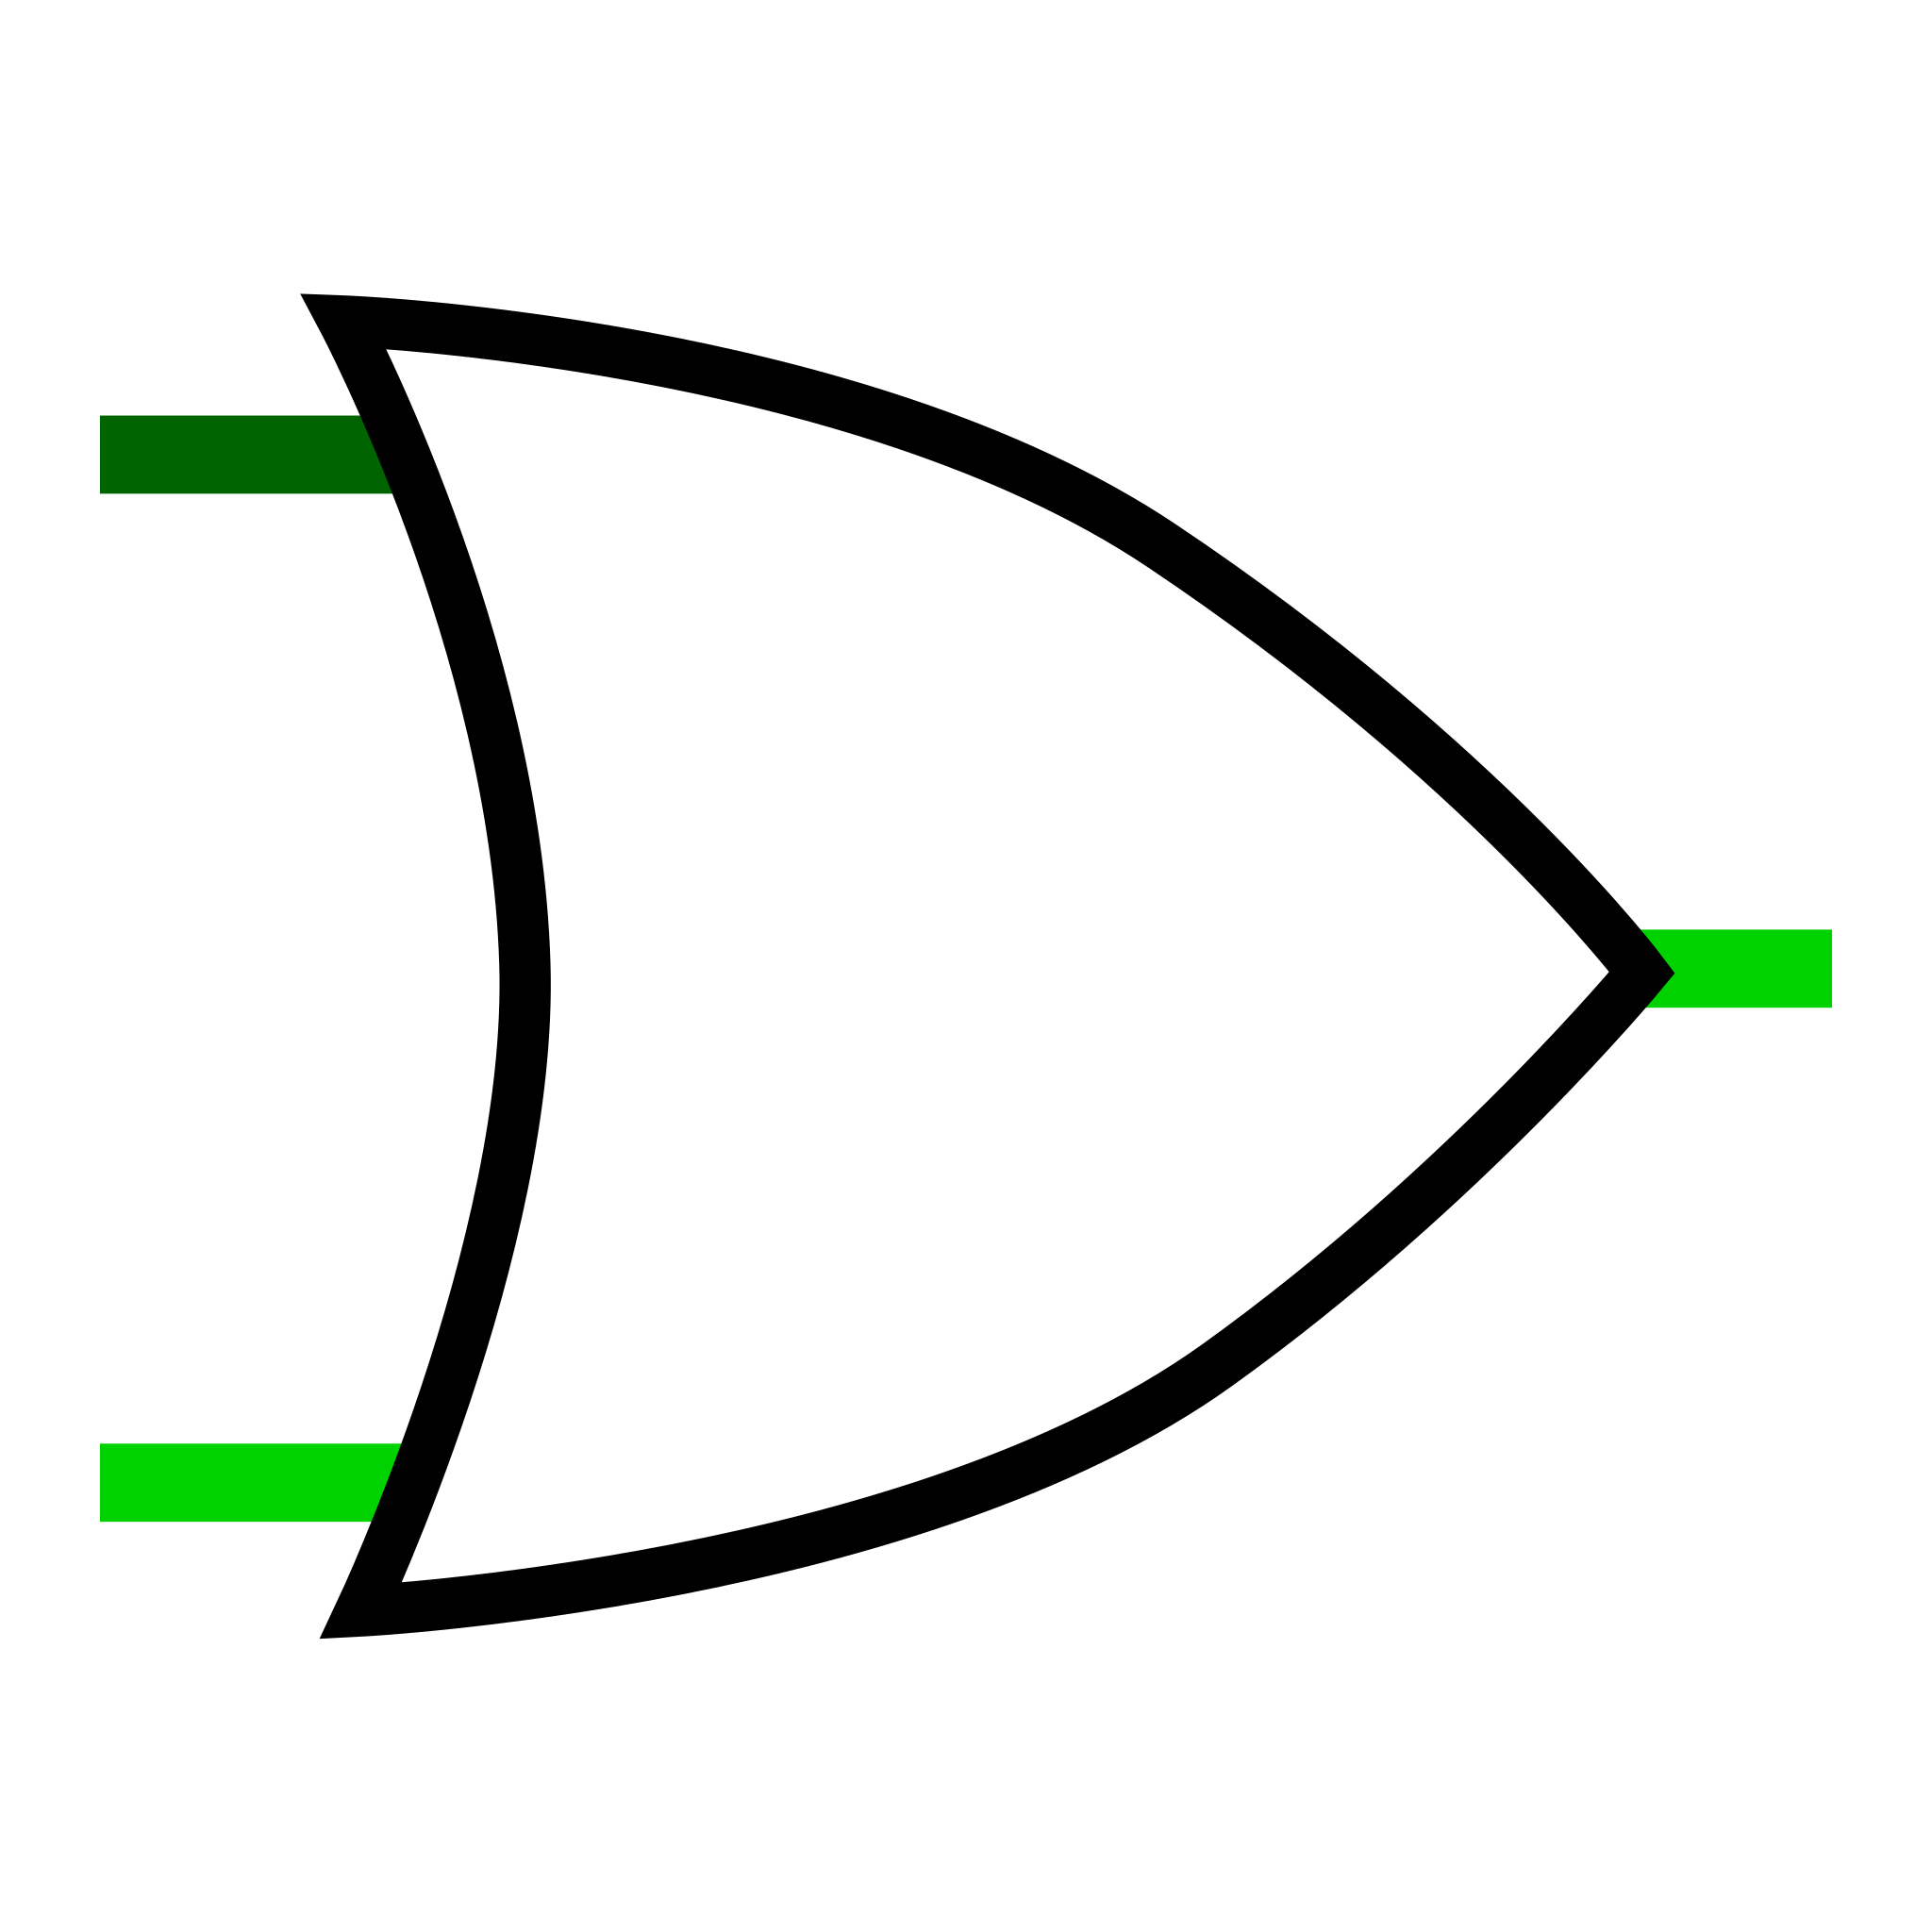
\includegraphics[scale=0.035]{conclusion/logisim.png}
\caption{
لوگوی نرم‌افزار
Logisim}
\end{figure}

نرم افزار دومی که با آن کار کردیم
Logisim
بود که این هم اوپن سورس است و ظاهر بسیار ساده‌ای دارد اما این یکی بر خلاف قبلی امکان شبیه‌سازی مدارها را به صورت در لحظه دارد به طوری که در حین اجرا نیز می‌توان ورودی‌ها را تغییر داد و نتیجه را درجا مشاهده کرد.
اما محدودیت این نرم‌افزار در کم بودن تنوع قطعات و ساده بودنش است به طوری که تنها گیت‌ها و برخی قطعات محدود را می‌توان در آن استفاده کرد.

\begin{figure}[h!]
\centering

\includegraphics[scale=0.3]{conclusion/proteus.png}
\caption{
لوگوی نرم‌افزار
Proteus}
\end{figure}

در انتها به نرم‌افزار
معروف
پولی فقط ویندوزی
Proteus
رسیدیم.
این نرم‌افزار ظاهر شلوغ و اعصاب خردکنی دارد اما در عوض بسیار کامل بوده و امکانات بسیار زیادی داردو همچنین تنوع قطعات آن بسیار فراوان است و گاه از زیاد بودن تنوع و مدل‌های یک قطعه اعصاب آزمایشگر را خرد می‌کند. 
اما در نهایت این تنوع و امکانات زیاد و امکان شبیه‌سازی بسیار خود آن باعث شده برای اکثر مدارها فراتر از نیاز آزمایشگر باشد.